\documentclass{article}
\PassOptionsToPackage{numbers,compress}{natbib}
\usepackage{lipsum}

% \usepackage{neurips_2021}
\usepackage[preprint]{neurips_2021}
% \usepackage[final]{neurips_2021}

\usepackage[T1]{fontenc}
\usepackage[latin1]{inputenc}
\usepackage{url}

\usepackage{hyperref}
\hypersetup{
    colorlinks=true,
    linkcolor=black,
    filecolor=blue,
    citecolor=blue,      
    urlcolor=cyan,
}

\usepackage{graphicx,xcolor,float}
\graphicspath{{./figures/}{docs/figures/}}

\usepackage{booktabs,amsmath,amsfonts}
\usepackage{nicefrac,microtype}

\usepackage{caption,subcaption}
\renewcommand\thesubfigure{\Alph{subfigure}}

\usepackage[ruled,vlined]{algorithm2e}
\numberwithin{equation}{section}
\numberwithin{figure}{section}



\title{Parameter Inference\\with Bifurcation Diagrams}
\author{
        Gregory Szep\\King's College London\\London, WC2R 2LS\\
        \texttt{gregory.szep@kcl.ac.uk}
    \And
        Attila Csik\'asz-Nagy\\King's College London\\London, WC2R 2LS\\
        \texttt{attila.csikasz-nagy@kcl.ac.uk}
    \And
        Neil Dalchau\\Microsoft Research Cambridge\\Cambridge, CB1 2FB\\
        \texttt{ndalchau@microsoft.com}
}

\begin{document}
\newcommand{\rates}{F_{\theta}}
\newcommand{\Det}{\Delta_{\theta}}
\newcommand{\tangent}{T_{\theta}}

\newcommand{\predictions}{\mathcal{P}}
\newcommand{\targets}{\mathcal{D}}
\newcommand{\loss}{L}

\newcommand{\Reals}{\mathbb{R}}
\maketitle
\begin{abstract}
    Estimation of parameters in differential equation models can be achieved by applying learning algorithms to time-series data. However, sometimes it is only possible to measure qualitative changes of a system in response to a controlled condition. In dynamical systems theory, such change points are known as \textit{bifurcations} and lie on a function of the controlled condition called the \textit{bifurcation diagram}. In this work, we propose a gradient-based semi-supervised approach for inferring the parameters of differential equations that produce a user-specified bifurcation diagram. The cost function contains a supervised error term that is minimal when the model bifurcations match the specified targets and an unsupervised bifurcation measure which has gradients that push optimisers towards bifurcating parameter regimes. The gradients can be computed without the need to differentiate through the operations of the solver that was used to compute the diagram. We demonstrate parameter inference with minimal models which explore the space of saddle-node and pitchfork diagrams and the genetic toggle switch from synthetic biology. Furthermore, the cost landscape allows us to organise models in terms of topological and geometric equivalence.
\end{abstract}


\section{Introduction}

Inverse problems \cite{Abdulla2009InverseBiology} arise in biology and engineering in settings when the model is not fully known and the desire is to match model behaviour to a given set of observations. This helps systematically guide both model and experimental design. The collected observations, however, are often indirectly proportional to the variables defined in the model; in microscopy, for example, data are reported in arbitrary fluorescence units allowing the observer to shift and scale data arbitrarily. The model, on the other hand, describes the dynamics of concentrations of relevant proteins. Furthermore, the observed qualitative changes in response to changes in experimental conditions are more robust and reproducible across studies than the quantitative details. For example, several studies are likely to agree that the human immune system activates above a threshold concentration of a pathogen and deactivates at a lower threshold concentration, but may disagree on the exact quantities of the thresholds or the magnitudes of the immune response. Bifurcation theory provides us a framework for studying these qualitative changes in a manner that is independent of quantitative details. The emerging picture suggests that identification of the qualitative behaviour -- the bifurcation diagram -- should precede any attempt at inferring other properties of a system \cite{Stumpf2019ParameterBifurcations}.

Inferring the parameters of a model directly from a bifurcation diagram is difficult because it is not obvious how one should change the parameters to create a bifurcation. It could even be impossible for the model to bifurcate in the manner desired. Several approaches exist to place bifurcations to desired locations once a manifold is present \cite{Iwasaki1997AnType,Lu2006InverseSystems,Dobson2004DistanceBifurcations} yet typically resort to sampling techniques to search for them in the first place \cite{Chickarmane2005BifurcationTool,Conrad2006BifurcationClock}. Progress has been made is cases where model structure and stability conditions are used to refine the search space \cite{Otero-Muras2018Optimization-basedModels,Otero-Muras2014ACurves} yet the resulting objectives are still not explicit in the bifurcation targets and also not differentiable. A scalable method for navigating the space of bifurcation diagrams would enable design of differential equations with high-level qualitative constraints. Furthermore one could begin organising models according to qualitatively distinct behaviours.

Back-propagation through differential equation solvers has been a breakthrough over the past couple of years \cite{Chen2018NeuralEquations,Rackauckas2019DiffEqFlux.jl-AEquations} that enabled scalable parameter inference for differential equations from trajectory data. Although one could use trajectory data to create the aforementioned qualitative constraints \cite{Ranciati2017BayesianParameters,Khadivar2021LearningBifurcations} this would entail over-constraining information originating from the kinetics and dynamical transients of the model. Furthermore, such data usually does not contain sufficient information about dynamical transients in order to identify kinetic parameters. Techniques for back-propagating through implicit equation solvers have also been developed \cite{Look2020DifferentiableLayers,Bai2019DeepModels} although to the best of the authors' knowledge have not been applied to bifurcation diagrams at the time of writing this paper.

In this work, we propose a gradient-based semi-supervised approach for inferring the parameters of differential equations that produce a user-specified bifurcation diagram. The bifurcation diagram encodes high-level qualitative information defined by state space structures, rather than kinetics. Drawing inspiration from implicit layers \cite{Look2020DifferentiableLayers,Bai2019DeepModels} to calculate gradients we find that their computation shares the same  complexity as the algorithm used to calculate the bifurcation diagram. The compute the diagram we use a predictor-corrector method called deflated pseudo-arclength continuation \cite{Farrell2016TheDiagrams,Veltz2019PseudoArcLengthContinuation.jl} developed for partial differential equations. In the case of partial differential equations the computational complexity of calculating a single bifurcation diagram is not bounded since superpositions of localised solutions may give rise to uncountably many branches \cite{Avitabile2010ToEquation}. The complexity of computing a single branch, however, is bounded by the complexities of the chosen eigenvalue solver and corrector, and further decreased by adaptive stepping procedures \cite{Aruliah2016AlgorithmContinuation}.

We find that the cost function landscape contains basins that not only allow us to synthesise models with a desired bifurcation diagram but also allow us to organise models in terms of topological and geometric equivalence. We discuss the relevance of this in model selection. In summary, our paper has the following main contributions:

\begin{itemize}
    \item An end-to-end differentiable method for searching for bifurcations and then matching them to user-specified target locations
    \item Implementation of the method in Julia package leveraging automatic differentiation tooling
    \item Leveraging the cost landscape for a novel way of organising differential equation models in terms of geometric and topological equivalence
\end{itemize}

\subsection{Preliminaries}

Suppose we collected observations along a scalar control condition $p\in\Reals$ and conclude that there are specific values of $p$ for which there are qualitative changes in system behaviour. Let $\targets$ be the set of those values and let us hypothesise that these transitions occur due to bifurcations in the dynamics that drive the underlying mechanism. Let us model the mechanism with a parameterised set of differential equations for states $u\in\Reals^N$ with a vector function $\rates$ in a parameter space $\theta\in\Reals^M$.

For the purposes of introducing this work, we will consider the simplest class of bifurcations known as \textit{co-dimension one} bifurcations, that do not include limit cycles. Therefore $\targets$ should contain conditions for which we hypothesise changes in multi-stable behaviour. Let the equations be
\begin{align}
	\frac{\partial u}{\partial t}=\rates(u,p)
	\qquad\mathrm{where}\quad
	\rates : \Reals^{N+1}\rightarrow\Reals^N
	\label{eq:model}
\end{align}

In the context of the differential equations, a co-dimension one bifurcation can be defined by a set of conditions on the determinant of the Jacobian $\Det$. The determinant of the Jacobian quantifies the rate at which trajectories in a local patch of state-space $u\in\Reals^N$ converge or diverge. The determinant approaching zero means that the dynamics of the system is slowing down, which is an important indicator for the onset of a transition between qualitative behaviours. Furthermore, the slowing down must necessarily be followed by breakdown of stability; for this to be true it is sufficient to require that the determinant cross zero with a finite slope, meaning that its directional derivative along the diagram $\frac{d}{ds}\Det$ is not zero. The set of predicted values for the control condition $\predictions(\theta)\subset\Reals$ at which bifurcations occur are defined as
\begin{align}
	\predictions(\theta):=\left\{\,
	p\,\,\exists\,\,u:\,\,\rates(u,p)=0,\,\,\Det=0,
	\,\, \frac{d}{ds}\Det\neq0
	\,\right\}
	\label{eq:predictions}
\end{align}
 Figure \ref{fig:minimal-models} shows minimal models that explore the space of saddle-nodes $\rates(u,p) = p + \theta_{1}u+\theta_{2}u^3$ and pitchforks $\rates(u,p) = \theta_{1} + p u+\theta_{2}u^3$. Indeed the predictions $\predictions(\theta)$ are defined by zero crossings in the determinant with a finite slope. The location of these crossings in general may not match the targets $\targets$.

For a given set of parameters $\theta$ one could compute the set of predicted bifurcations $\predictions(\theta)$ using parameter continuation methods \cite{Veltz2019PseudoArcLengthContinuation.jl,Farrell2016TheDiagrams}. Our goal is to find optimal parameters $\theta^*$ that match predictions $\predictions(\theta^*)$ to specified targets $\targets$. We must design a suitable cost function $\loss$ so that
\begin{align}
    \theta^* := \mathrm{argmin}_{\theta} \loss(\theta|\targets)
    \label{eq:optimal-theta}
\end{align}
The optimal $\theta^*$ is not expected to always be unique, but is in general a manifold representing the space of qualitatively equivalent models. The cost function $\loss$ must have some distance measure between the two sets $\predictions(\theta)$ and $\targets$ with a bias that encourages equivalent set sizes $|\predictions(\theta)|=|\targets|$. This is especially important in the case where there are no predictions $|\predictions(\theta)|=0$.

\begin{figure}
\centering
\setlength\unitlength{1cm}
{\phantomsubcaption\label{fig:saddle-node}}
{\phantomsubcaption\label{fig:pitchfork}}
\includegraphics[width=6cm]{saddle-node}
\begin{picture}(0,0) \put(-5.8,10){\subref{fig:saddle-node}} \end{picture}
\includegraphics[width=6cm]{pitchfork}
\begin{picture}(0,0) \put(-5.8,10){\subref{fig:pitchfork}} \end{picture}
\caption{Saddle-node model \ref{fig:saddle-node} $\rates(u,p) = p + \theta_{1}u+\theta_{2}u^3$ and pitchfork model \ref{fig:pitchfork} $\rates(u,p) = \theta_{1} + p u+\theta_{2}u^3$ with $\theta=(5/2,-1),(1/2,-1)$ and targets $\targets=\{-1,1\},\{0\}$ respectively. Lighter shades indicate the determinant crossing zero at locations $\predictions(\theta)$ giving rise to unstable solutions}
\label{fig:minimal-models}
\end{figure}

\section{Proposed Method}
\subsection{Semi-supervised Cost Function}

\begin{figure}
    \centering
    \includegraphics[width=7cm]{bifurcation-measure}
    \caption{Bifurcation measure $\measure(s)$ and determinant $\Det$ along two different bifurcation curves demonstrating how maximising the measure along the curve maintains the existing bifurcation marked by a circle, while encouraging new bifurcations marked by stars}
    \label{fig:measure}
\end{figure}

In order for predicted bifurcations $p(\theta)\in\predictions(\theta)$ to match targets $p'\in\targets$ we need to evaluate an error term $|p(\theta)-p'|$. We expect this term to be some mean over the targets $\targets$ and predictions $\predictions(\theta)$. We choose a geometric mean over the predictions and an arithmetic mean over targets to account for cases where $|\predictions|\neq|\targets|$ and discourage multiple predictions matching the same target in cases where $|\predictions|\geq|\targets|$. This term only zero when each target is matched by at least one prediction
\begin{align}
    \frac{1}{|\targets|}\sum_{p'\in\targets}
    \prod_{p(\theta)\in\predictions(\theta)}|p(\theta)-p'|
    ^{\frac{1}{|\predictions|}}
    \label{eq:error}
\end{align}
We can see from Figures \ref{fig:minimal-models} and definitions \eqref{eq:predictions} that predictions $p(\theta)$ can be identified by looking for points along the curve where the determinant $\Det=0$. Meanwhile the directional derivative along the bifurcation curve is finite $\frac{d}{ds}\Det\neq 0$. Using these quantities we can define a positive semi-definite measure $\measure(u,p)$ of zero crossings in the determinant along the bifurcation curve. Figure \ref{fig:measure} demonstrates this measure is maximal at bifurcation at locations $p(\theta)$ and has finite gradients in non-bifurcating regimes. The total bifurcation measure $\Psi(\theta)$ is defined as
\begin{align}
    \Psi(\theta):=\frac{
        \int_{\rates(u,p)=0}\!
        \measure(u,p)\,\mathrm{d}u\mathrm{d}p
    }{
        \int_{\rates(u,p)=0}\!\
        \mathrm{d}u\mathrm{d}p
    }
    \quad\mathrm{where}\quad
    \measure(u,p):=
    \left(1+\left|\frac{\Det}{\frac{d}{ds}\Det}\right|\right)^{-1}
    \label{eq:measure}
\end{align}
Here we denote $\int_{\rates(u,p)=0}\mathrm{d}u\mathrm{d}p$ as the sum of the line integrals in $(u,p)\in\Reals^{N+1}$ defined by the level set $\rates(u,p)=0$. The measure $\measure(u,p)$ is one at bifurcation points and goes to zero an odd number of times between bifurcations. This is because $\Det$ must eventually turn around in order to return back to zero, resulting in the directional derivative $\frac{d}{ds}\Det$ going to zero and hence the measure $\measure(u,p)$ going to zero for each turning point. While the calculation of the determinant is straightforward, its directional derivative is not. Fortunately, a tangent field representation of the bifurcation curve allows us to compute this derivative implicitly; see Appendix \ref{appendix:tangent-fields} for details.

As the determinant $\Det$ diverges we approach regimes far away from any closest bifurcation and hence $\measure(u,p)\rightarrow0$. We would still like to have non-zero gradients with respect to $\theta$ in this regime, and therefore $\measure(u,p)$ was designed to go to zero slowly. The total measure $\Psi(\theta)$ is normalised such that $\Psi(\theta)\rightarrow1$ in the regimes where the controlled condition region $p$ is densely packed with bifurcations. The measure $\measure(u,p)$ is also invariant under certain classes of transformations on $\rates(u,p)$ which do not change bifurcation locations, proofs of which are provided in Appendix \ref{appendix:measure}. The total measure $\Psi(\theta)$ is added to the supervised term as if it were a likelihood; this defines the semi-supervised cost function as
\begin{align}
    \loss(\theta|\targets):=
    \big(|\predictions|-|\targets|\big)\,\,\lambda \log\Psi(\theta)+
    \frac{1}{|\targets|}\sum_{p'}
    \prod_{p(\theta)}|p(\theta)-p'|
    ^{\frac{1}{|\predictions|}}
    \label{eq:loss}
\end{align}
The pre-factor $|\targets|-|\predictions|$ in the unsupervised term ensures that the gradients are always pushing optimisers towards a state where $|\targets|=|\predictions|$. This can be seen as a step-wise annealing of the unsupervised term until the desired state is reached. Note that in while individual bifurcations $p(\theta)$ depend smoothly on $\theta$, the total number of predictions $|\predictions|$ does not have gradient contributions with respect to $\theta$. We can safely drop the dependency in the prediction counter and now proceed in taking gradients with respect to $\theta$ knowing that the only dependencies we need to track are for individual bifurcations $p(\theta)$ and total measure $\Psi(\theta)$
\begin{align}
    \frac{\partial\loss}{\partial\theta}=
    \big(|\predictions|-|\targets|\big)\,\lambda\,
    \frac{\partial \Psi}{\partial\theta}\Psi(\theta)^{-1}+
    \frac{1}{|\targets||\predictions|}\sum_{p'}
    \prod_{p(\theta)}|p(\theta)-p'|^{\frac{1}{|\predictions|}}
    \sum_{p(\theta)}\frac{\partial p}{\partial\theta}\left(p(\theta)-p'\right)^{-1}
    \label{eq:gradient-loss}
\end{align}
In a similar vein to back-propagation through neural differential equations \cite{Chen2018NeuralEquations} we would like to be able to calculate the gradient $\frac{\partial\loss}{\partial\theta}$ without having to differentiate through the operations of the solver that finds the bifurcation curve $\rates(u,p)=0$ and the bifurcation locations $p(\theta)$. To calculate the gradient of the measure $\frac{\partial \Psi}{\partial\theta}$ we need to differentiate line integrals that depend on $\theta$. Fortunately this can be done by the application of the generalised Leibniz integral rule, details of which can be found in Appendix \ref{appendix:space-curve}.

The gradient of the bifurcation points $\frac{\partial p}{\partial\theta}$ is found by application of the implicit function theorem to a vector function $G_{\theta}:\Reals^{N+1}\rightarrow\Reals^{N+1}$ whos components represent the two constraints $\rates(u,p)=0$ and $\Det=0$. By following a similar strategy to that used by implicit layers \cite{Look2020DifferentiableLayers} we yield an $(N+1)\times M$ Jacobian representing a deformation field \cite{Jos2011OnSurface} for each $\theta$ direction. The gradient we are looking for becomes
\begin{align}
    \frac{\partial p}{\partial\theta} = -\hat{p}\cdot\left.\frac{\partial G_{\theta}}{\partial (u,p)}^{-1}
    \frac{\partial  G_{\theta}}{\partial\theta}\right|_{G_{\theta}(u,p)=0}
    \quad\mathrm{where}\quad
    G_{\theta}(u,p):=\begin{bmatrix}\rates(u,p)\\\Det\end{bmatrix}
    \label{eq:gradient-bifurcation}
\end{align}
Here $\hat{p}$ is a unit vector in $(u,p)\in\Reals^{N+1}$ that picks out the deformations along the $p$-direction. If we wanted to place the bifurcation at target steady state $u'$ as well as target control condition $p'$ we would use the full $(N+1)\times M$ deformation matrix. Calculation of this matrix involves inverting an $(N+1)\times(N+1)$ Jacobian $\frac{\partial G_{\theta}}{\partial(u,p)}$. The determinant of this Jacobian goes to zero in the degenerate case where $\frac{d}{ds}\Det=0$. This further justifies our choice for measure $\Psi(\theta)$ which discourages the degenerate case.

The cost function is piece-wise smooth and differentiable with undefined gradients only in parameter contours where the number of predictions $|\predictions|$ changes; this is when $\Psi(\theta)$ is undefined and the inverse of $\frac{\partial G_{\theta}}{\partial (u,p)}$ does not exist. Given a set of solutions to $\rates(u,p)=0$ and locations $p(\theta)$ the gradient $\frac{\partial\loss}{\partial\theta}$ can evaluated using automatic differentiation methods without needing to back-propagate through the solver that obtained the level set $\rates(u,p)=0$ in the forward pass.

\section{Experiments \& Results}

\subsection{Minimal Models}
Figures \ref{fig:saddle-node:results} and \ref{fig:pitchfork:results} show example optimisations of $(\theta_1,\theta_2)$ for the minimal saddle-node and pitchfork models respectively. The magnitude of the correction factor $\lambda=0$ when bifurcations are present and $\lambda\neq0$ otherwise. Optimisation trajectories approach lines of global minima in the cost function, which represent a set of geometrically equivalent models, depicted in the right panels. Two bifurcation curves are geometrically equivalent if the number, type and locations of bifurcations match.

We can see that the geometrically equivalent lines are contained within larger basins defined by $\lambda=0$ where the correct number and type of bifurcations are present $p\in\Omega$, but do not match the locations of targets $\targets$. All models within this basin are in some sense topologically equivalent. This hierarchical classification allows us to identify the set of models that satisfy observed qualitative behaviour \cite{Stumpf2019ParameterBifurcations} before any attempt at inferring kinetic parameters, which is done by choosing a model along the line of geometrically equivalent models.

Optimisation trajectories for the two minimal models appear mostly circumferential. This is because the models were set up such that the radial direction from the origin in $\theta$ space mostly scale kinetics whereas the circumferential direction changes the bifurcation topology. This suggests that the gradients of our cost function seek to change model geometry over kinetics.

\begin{figure}
\centering
\includegraphics[width=6cm]{saddle-landscape.png}
\includegraphics[width=6cm]{saddle-optima.png}
\caption{Saddle-node model $\rates(u,p) = p + \theta_{1}u+\theta_{2}u^3$ optimised with respect to targets $\targets=\{-1,1\}$ in observation region $\Omega\in[-2,2]$. The right panel shows bifurcations diagrams for the three optima marked by stars on the left panel. The optimisation trajectories in white follow the gradient of the cost, approaching the black line of global minima in the left panel}
\label{fig:saddle-node:results}
\end{figure}

\begin{figure}
\centering
\includegraphics[width=6cm]{pitchfork-landscape.png}
\includegraphics[width=6cm]{pitchfork-optima.png}
\caption{Pitchfork model $\rates(u,p) = \theta_{1} + u p +\theta_{2}u^3$ optimised with respect to targets $\targets=\{0\}$ in observation region $\Omega\in[-5,5]$. The right panel shows bifurcations diagrams for the three optima marked by stars on the left panel. The optimisation trajectories in white follow the gradient of the cost, approaching the black lines of global minima in the left panel}
\label{fig:pitchfork:results}
\end{figure}

\subsection{Genetic Toggle Switch}
In this section we optimise a model where the states share a Hill function relationship with cooperatively $n=2$; these models often emerge from mass action kinetics and are used to model species concentrations. After re-scaling the equations governing the dynamics of concentrations, the simplified equations for state $u_$ and $u_2$ become 
\begin{equation}
    \partial_t u_1 = \frac{ a_1 + (p u_2)^2}{ 1 + (p u_2)^2 } - \mu_1 u_1 \quad
    \partial_t u_2 = \frac{ a_2 + (k u_1)^2}{ 1 + (k u_1)^2 } - \mu_2 u_2
    \label{eq:two-state}
\end{equation}
where $a_k$ are 
 the  we can recover both activator and inhibitor relationships.
Figure \ref{fig:two-state-optima} shows a UMAP embedding of the optimal parameter basins, represented as point clouds. 16 distinct clusters are obtained using DBSCAN. Each cluster corresponds to a kinetically different model regions that are qualitatively equivalent. See Appendix \ref{appendix:clusters} for models that represent the centroid of each cluster.
 
\begin{figure}
\centering
\includegraphics[width=11cm]{two-state-optima}
\caption{Optimal parameter estimates $\theta^*$ for the two state model \eqref{eq:two-state} for the targets $\targets=\{4,5\}$ reveal two clusters of qualitatively different regimes: mutual activation and mutual inhibition. }
\label{fig:two-state-optima}
\end{figure}
 
\section{Conclusion \& Broader Impact | \textit{in progress}}
\begin{itemize}
    \item Taking steps towards an efficient and single method for searching and matching bifurcations
    \item A demonstrating of the powerful combination of differential geometry and implicit layers
    \item Future directions include extending this routine for Hopf bifurcations and PDEs
    \item Computational limitations
\end{itemize}

% \section*{Checklist}
% \begin{enumerate}

\item For all authors...
\begin{enumerate}
  \item Do the main claims made in the abstract and introduction accurately reflect the paper's contributions and scope?
    \answerYes{}
  \item Did you describe the limitations of your work?
    \answerYes{Implementation only covers co-dimension one bifurcations. Does not scale well for PDEs. See discussion in Section \ref{}}
  \item Did you discuss any potential negative societal impacts of your work?
    \answerNA{}
  \item Have you read the ethics review guidelines and ensured that your paper conforms to them?
    \answerYes{}
\end{enumerate}

\item If you are including theoretical results...
\begin{enumerate}
  \item Did you state the full set of assumptions of all theoretical results?
    \answerNA{This paper applies existing theorems. See Section \ref{section:method}}
	\item Did you include complete proofs of all theoretical results?
    \answerNA{We include derivations to guide the reader in Appendices}
\end{enumerate}

\item If you ran experiments...
\begin{enumerate}
  \item Did you include the code, data, and instructions needed to reproduce the main experimental results (either in the supplemental material or as a URL)?
    \answerYes{All figures are unit tests in the GitHub repository for \texttt{BifurcationFit.jl}}
  \item Did you specify all the training details (e.g., data splits, hyperparameters, how they were chosen)?
    \answerYes{ADAM was used with various hyper-parameters}
	\item Did you report error bars (e.g., with respect to the random seed after running experiments multiple times)?
    \answerYes{See Figure \ref{fig:scaling} and }
	\item Did you include the total amount of compute and the type of resources used (e.g., type of GPUs, internal cluster, or cloud provider)?
    \answerYes{See Figure \ref{fig:scaling}}
\end{enumerate}

\item If you are using existing assets (e.g., code, data, models) or curating/releasing new assets...
\begin{enumerate}
  \item If your work uses existing assets, did you cite the creators?
    \answerYes{\cite{Veltz2019PseudoArcLengthContinuation.jl,Revels2016Forward-ModeJulia,Flux}}
  \item Did you mention the license of the assets?
    \answerNo{All assets have been release under MIT}
  \item Did you include any new assets either in the supplemental material or as a URL?
    \answerYes{All code available under \texttt{github.com/gszep/BifurcationFit.jl} }
  \item Did you discuss whether and how consent was obtained from people whose data you're using/curating?
    \answerNA{}
  \item Did you discuss whether the data you are using/curating contains personally identifiable information or offensive content?
    \answerNA{}
\end{enumerate}

\item If you used crowdsourcing or conducted research with human subjects...
\begin{enumerate}
  \item Did you include the full text of instructions given to participants and screenshots, if applicable?
    \answerNA{}
  \item Did you describe any potential participant risks, with links to Institutional Review Board (IRB) approvals, if applicable?
    \answerNA{}
  \item Did you include the estimated hourly wage paid to participants and the total amount spent on participant compensation?
    \answerNA{}
\end{enumerate}

\end{enumerate}

\bibliography{refs}
\bibliographystyle{ieeetr}

\section*{Appendix}
\appendix
\section{Bifurcation Diagrams as Tangent Fields}
\label{appendix:tangent-fields}

Let each component of the vector function $\rates$ in the model \eqref{eq:model} implicitly define a surface embedded in $\Reals^{N+1}$. Let's assume that the intersection of these $N$ surfaces exists and is not null or degenerate, then the steady states of \eqref{eq:model} must be a set of one dimensional space curves in $z\in\Reals^{N+1}$ defined by
\begin{align}
    \rates(z) = 0
\end{align}
\begin{figure}[H]
\centering
\includegraphics[width=5cm]{implicit-surfaces}
\caption{Two implicit surfaces $f_{\theta}(z)=0$ and $g_{\theta}(z)=0$ in $\mathbb{R}^3$ intersecting to form a space curve which is tangent to field $\tangent(z)$ and perpendicular to gradients $\partial_{z}f_{\theta}$ and $\partial_{z}g_{\theta}$}
\label{fig:implicit-surfaces}
\end{figure}
An expression for the field $\tangent(z)$ tangent to the set of curves would allow us to take derivatives and integrals along the bifurcation curve. This is exactly what we need to do to evaluate our cost function \ref{eq:loss}. Fortunately the tangent field can be constructed by ensuring it is perpendicular to the gradient $\partial_z$ of each component of $\rates$ as illustrated by an example two component system in Figure \ref{fig:implicit-surfaces}. The tangent field $\tangent(z)$ can be constructed perpendicular to all gradient vectors using the properties of the determinant \cite{Goldman2005CurvatureSurfaces}
\begin{align}
    \tangent(z):=
    \label{eq:tangent-field}
    \left|\begin{matrix}
        \hat{z} \\
        \,\partial_{z}\rates\,
    \end{matrix}\right|
    \qquad\tangent : \Reals^{N+1}\rightarrow\Reals^{N+1}\\
    =\sum_{i=1}^{N+1}\hat{z}_{i}(-1)^{i+1} \left|\frac{\partial \rates}{\partial(z\setminus z_{i}) }\right|
\end{align}
where $\hat{z}$ is a collection of unit basis vectors in the $\Reals^{N+1}$ space and $\partial_{z}\rates$ is an $N\times(N+1)$ rectangular Jacobian matrix of partial derivatives and $z\setminus z_{i}$ denotes the $N$ dimensional vector $z$ with component $z_{i}$ removed. This construction ensures perpendicularity to any gradients of $\rates$
\begin{align}
    \tangent(z)\cdot\partial_z f_{\theta} =
    \left|\begin{matrix}
        \partial_z f_{\theta} \\
        \,\partial_{z}\rates\,
    \end{matrix}\right|
    \quad =0 \quad\forall f_{\theta}\in \rates
\end{align}
since the determinant of any matrix with two identical rows or columns is zero. Note that the tangent field $\tangent(z)$ is actually defined for all values of $z$ where adjacent field lines trace out other level sets where $\rates(z)\neq0$. Furthermore deformations with respect to $\theta$ are always orthogonal to the tangent
\begin{align} % \todo{numerically true. analytic proof?}
    \tangent(z)\cdot\frac{d\tangent}{d\theta}=0
\end{align}
\begin{figure}
\centering
\includegraphics[width=13cm]{determinant-field}
\caption{Left/Right : Determinant $\Det$ and tangent field $\tangent(z)$ for the saddle-node/pitchfork models for some set values of $\theta$ revealing that $\Det=0$ defines bifurcations}
\label{fig:determinant-field}
\end{figure}
Figure \ref{fig:determinant-field} shows how the bifurcation curve defined by $\rates(z)=0$ picks out one of many level sets or traces in tangent field $\tangent(z)$ for the saddle and pitchfork. The tangent field $\tangent(z)$ can always be analytically evaluated by taking the determinant in \eqref{eq:tangent-field}. We will proceed with calculations on $\tangent(z)$ in the whole space $z$ and pick out a single trace by solving $\rates(z)=0$ later. For our two models
\begin{align}
    \underset{\mathrm{saddle-node\,\,model}}{
    \tangent(z)=\hat{u}-(\,3\theta_2 u^2+\theta_1\,)\,\hat{p}}
    \qquad\qquad
    \underset{\mathrm{pitchfork\,\,model}}{
    \tangent(z)=u\hat{u}-(\,3\theta_2 u^2+p\,)\,\hat{p}}
    \label{eq:tangent-field-examples}
\end{align}
Figure \ref{fig:determinant-field} reveals that $\Det=0$ is also a level set and that the intersection with level set $\rates(z)=0$ defines the bifurcations at specific parameter $\theta$. In this particular setting we can see that the tangent field $\tangent(z)$ only folds when $\Det=0$. Plotting the value of the determinant along $\rates(z)=0$ from Figure \ref{fig:determinant-field} would give rise to Figures \ref{fig:minimal-models}. The directional derivative of the determinant $\Det$ along the tangent field $\tangent(z)$ is defined as
\begin{align}
    \frac{d}{ds}\Det := \hat{\tangent}(z) \cdot \frac{\partial}{\partial z}\Det 
\end{align}
where $\hat{\tangent}(z)$ is the unit tangent field.

\section{Bifurcation Measure Properties}
\label{appendix:conditions}
Consider a vector $v(s)\in\Reals^N$ parametrised by $s\in\Reals$ that is tangent to an equilibrium manifold defined by $\rates(u)=0$. The conditions for a non-degenerate static bifurcation at $s^*$ along such a tangent can be expressed in terms of an eigenvalue $\lambda(s)$ of the state-space Jacobian crossing zero with a finite slope. A bifurcation exists at $s^*$ if
\begin{align}
    \frac{\partial\rates}{\partial u}v(s)=\lambda(s) \,v(s)
    \quad\exists\lambda:\quad
    \left.\lambda(s)\right|_{s=s^*}=0
    \qquad
    \left.\frac{d\lambda}{ds}\right|_{s=s^*}\neq 0
    \label{eq:conditions}
\end{align}
These conditions are necessary and sufficient for a non-degenerate static local breakdown of stability. For now we do not consider dynamic bifurcations involving limit cycles or imaginary parts of eigenvalues and restrict $\lambda\in\Reals$. Cases where both $\left.\lambda(s)\right|_{s=s^*}=0$ and $\left.\frac{d\lambda}{ds}\right|_{s=s^*}=0$ require investigation into higher order derivatives $\frac{d^n\lambda}{ds^n}$. These are the cases we refer to as \emph{degenerate} and are not considered here.

Instead of considering conditions on each eigenvalue individually it is possible to use the determinant of the state-space Jacobian to detect whether the conditions \eqref{eq:conditions} are satisfied. The determinant can be expressed as the product of eigenvalues
\begin{equation}
    \Det=\prod_{n=1}^N\lambda_n(s)
    \label{eq:determinant}
\end{equation}
Applying the product rule when differentiating yields
\begin{align}
    \frac{d}{ds}\Det&=
    \sum_{n=1}^N\frac{d\lambda_n}{ds}\prod_{n'\neq n}\lambda_{n'}(s)\\
    &=\Det\sum_{n=1}^N\frac{d\lambda_n}{ds}\lambda_{n}(s)^{-1}
\end{align}
Substituting this expression into measure \eqref{eq:measure}
\begin{equation}
    \measure(s)=
    \left(1+\left|\sum_{n=1}^N\frac{d\lambda_n}{ds}\lambda_{n}(s)^{-1}\right|^{-1}\right)^{-1}
\end{equation}
Which implies the following
\begin{equation}
    \exists\lambda:\quad
    \begin{cases}
        \,\lambda(s)=0 \quad\frac{d\lambda}{ds}\neq 0\\
        \,\lambda(s)\neq0 \quad\frac{d\lambda}{ds}\rightarrow\pm\infty
    \end{cases}
    \implies
    \measure(s)=1
    \label{eq:measure-conditions}
\end{equation}
If there exists an eigenvalue that satisfies conditions \eqref{eq:conditions} then the measure is equal to one. The measure also approaches one in cases where the rate of change of an eigenvalue with respect to a manifold $s$ location  diverges while not crossing zero. This gives rise to finite gradients in the eigenvalue term in regimes far away from any bifurcation.

\section{Leibniz Rule for Space Curves}
\label{appendix:leibniz-rule}

Suppose there exists a one dimensional space curve $\mathcal{C(\theta)}$ embedded in $z\in\Reals^{N+1}$ whose geometry changes depending on input parameters $\theta\in\Reals^M$. This curve could be open or closed and changes in $\theta$ could change the curve topology as well. Let the function $\gamma_{\theta}:\Reals\rightarrow\Reals^{N+1}$ be a parametrisation of the position vector along the curve within a fixed domain $s\in\mathcal{S}$. Note that the choice of parametrisation is arbitrary and our results should not depend on this choice. Furthermore, if we parametrise the curve $\mathcal{C}(\theta)$ with respect to a fixed domain $\mathcal{S}$ the dependence on $\theta$ is picked up by the parametrisation $\gamma_{\theta}(s)$. We can write a line integral of any scalar function $L_{\theta}:\Reals^{N+1}\rightarrow\Reals$ on the curve as
\begin{align}
    L(\theta):=
    \int_\mathcal{C(\theta)}\! L_{\theta}(z)\,\mathrm{d}z
    =\int_\mathcal{S}\! L_{\theta}(z)\left|\frac{d\gamma_{\theta}}{ds}\right|\mathrm{d}s_{\,\,z=\gamma_{\theta}(s)}
\end{align}
where $\left|\frac{d\gamma_{\theta}}{ds}\right|$ is the magnitude of tangent vectors to the space curve and we remind ourselves that the integrand is evaluated at $z=\gamma_{\theta}(s)$. We would like to track how this integral changes with respect to $\theta$. The total derivative with respect to $\theta$ can be propagated into the integrand \cite{Flanders1973DifferentiationSign} as long as we keep track of implicit dependencies
\begin{align}
    \frac{dL}{d\theta} &=\int_\mathcal{S}
    \left|\frac{d\gamma_{\theta}}{ds}\right|
    \left(
        \frac{\partial L}{\partial\theta}+
        \frac{\partial L}{\partial z}\cdot
        \frac{dz}{d\theta}
    \right)
    +L_{\theta}(z)\frac{d}{d\theta}\left|\frac{d\gamma_{\theta}}{ds}\right|
    \mathrm{d}s_{\,\,z=\gamma_{\theta}(s)}
\end{align}
Here we applied the total derivative rule in the first term due to the implicit dependence of $z$ on $\theta$ through $z=\gamma_{\theta}(s)$. Applying the chain rule to the second term
\begin{align}
    \frac{d}{d\theta}\left|\frac{d\gamma_{\theta}}{ds}\right|=
    \left|\frac{d\gamma_{\theta}}{ds}\right|^{-1}
    \frac{d\gamma_{\theta}}{ds}\cdot\frac{d}{d\theta}
    \left(\frac{d\gamma_{\theta}}{ds}\right)
\end{align}
By choosing an $s$ that has no implicit $\theta$ dependence we can commute derivatives
\begin{align}
    \frac{d}{d\theta}\left(\frac{d\gamma_{\theta}}{ds}\right)
    = \frac{d}{ds}\left(\frac{d\gamma_{\theta}}{d\theta}\right)
    \quad\Rightarrow\quad
    \frac{d}{d\theta}\left|\frac{d\gamma_{\theta}}{ds}\right|=
    \left|\frac{d\gamma_{\theta}}{ds}\right|^{-1}
    \frac{d\gamma_{\theta}}{ds}\cdot\frac{d}{d s}
    \left(\frac{d\gamma_{\theta}}{d\theta}\right)
\end{align}
To proceed we note that the unit tangent vector can be written as an evaluation of a tangent field $\hat{T}_{\theta}(z)$ defined in the whole domain $z\in\Reals^{N+1}$ along the parametric curve $z=\gamma_{\theta}(s)$. The unit tangent field may disagree with the tangent given by $\frac{d\gamma_{\theta}}{ds}$ up to a sign
\begin{align}
    \left.\hat{\tangent}(z)\right|_{z=\gamma_{\theta}(s)}=
    \pm\left|\frac{d\gamma_{\theta}}{ds}\right|^{-1}\frac{d\gamma_{\theta}}{d s}
\end{align}
this leads to
\begin{align}
    \frac{d}{d\theta}\left|\frac{d\gamma_{\theta}}{ds}\right|=
    \left|\frac{d\gamma_{\theta}}{ds}\right|\left(
   \hat{\tangent}(z)\cdot\frac{\partial }{\partial z}\left(\frac{d\Gamma_{\theta}}{d \theta}\right)\cdot
   \hat{\tangent}(z)
    \right)_{z=\gamma_\theta(s)}
    \label{eq:divergence-term}
\end{align}
It is possible to find the normal deformation of the implicit space curves due to changes in $\theta$. This can be done by taking the total derivative of the implicit equation defining the level set
\begin{align}
    \frac{d\rates(z)}{d\theta}=\frac{\partial F}{\partial\theta}+
    \frac{\partial F}{\partial z}\cdot\frac{d z}{d \theta}
\end{align}
We can rearrange for $\frac{d z}{d \theta}$ using the Moore-Penrose inverse of the rectangular Jacobian matrix $\frac{\partial F}{\partial z}$ which appeared in equation \eqref{eq:tangent-field}. Since the level set is defined by $\rates(z)=0$ the total derivative along the level set $d\rates(z)=0$ and we arrive at an expression for the deformation field \cite{Jos2011OnSurface}
\begin{align}
    \frac{d z}{d \theta} = - \frac{\partial F}{\partial z}^\top
    \left(\,
        \frac{\partial F}{\partial z}\,\frac{\partial F}{\partial z}^\top
    \right)^{-1}
    \frac{\partial F}{\partial\theta}
\end{align}
The tangential component of the deformation field is not uniquely determined because there is no unique way of parametrising a surface. This is the subject of many computer graphics papers \cite{Jos2011OnSurface,Tao2016Near-IsometricTracking,Fujisawa2013CalculationInvariance}. We are however not interested in the continuous propagation of a mesh - as is the subject of those papers. In fact we are looking for a deformation field that is orthogonal to the tangent vector $\hat{\tangent}(z) \cdot\frac{d z}{d\theta} =0$ for the space curve, and therefore letting the tangential component of the deformation equal zero is a valid choice and we can it instead of the parametrised deformation
\begin{align}
    \frac{d \gamma_{\theta}}{d\theta} \rightarrow \frac{d z}{d\theta}
\end{align}
To summarise we now have the gradient of our line integral only in terms of the implicit function defining the integration region.
\begin{align}
    \frac{d L}{d\theta} =\int_{\rates(z)=0}
        \frac{\partial L}{\partial\theta}+
        \frac{\partial L}{\partial z}\cdot
        \varphi_{\theta}(z)
    +L_{\theta}(z)\,\,
    \hat{\tangent}(z)\cdot\frac{\partial \varphi}{\partial z}\cdot\hat{\tangent}(z)
    \,\mathrm{d}z\qquad\qquad\\
    \mathrm{where}\quad
    \hat{\tangent}(z):= \frac{\tangent(z)}{|\tangent(z)|}
    \qquad
    \tangent(z):=
    \left|\begin{matrix}
        \hat{z} \\
        \,\partial_{z}\rates\,
    \end{matrix}\right|
    \qquad
    \varphi_{\theta}(z) :=
- \frac{\partial F}{\partial z}^\top
    \left(\,
        \frac{\partial F}{\partial z}\,\frac{\partial F}{\partial z}^\top
    \right)^{-1}
    \frac{\partial F}{\partial\theta}
\end{align}
We have settled on choosing normal deformations which we will call $\varphi_\theta(z)$. The above result can be seen a the generalised Leibniz rule \cite{Flanders1973DifferentiationSign} for the case of line integration regions. The last integrand term can be seen as the divergence the vector field $\varphi_\theta(z)$ projected onto the one dimensional space curve.

\clearpage

\section{Application of Bifurcation Inference to a Complex Model}
\label{appendix:double-exclusive}

To demonstrate the wider reaching applicability of our method we optimise the \emph{double exclusive reporter} \cite{Grant2020InterpretationCircuit}, a synthetic gene circuit in \emph{E. coli} that was designed to exhibit a cusp bifurcation. The circuit behaviour is observed by measuring a fluorescent protein whose expression is controlled by transcription factors (regulatory proteins) LacI $(L)$ and TetR $(T)$, whose expression is in turn controlled by externally controllable \emph{input} signals $c_{6}$ and $c_{12}$. To apply the method, we consider one of the input signals be the control condition $c_{6}=p$, with the other packed together with the remaining 20 parameters into vector $\theta$. Once the optima $\theta^*$ have been obtained, we perform dimensionality reduction using \texttt{GigaSOM.jl} \cite{Kratochvil2020GigaSOM.jl:Datasets} so that the results can be visualised in a two dimensional embedding (Figure \ref{fig:double-exclusive-optima:parameters}).

The embedding reveals four optimal parameter regions. We find that, as with the two-state model in the main text \eqref{eq:two-state}, there are two qualitatively distinct regimes: mutual activation (region 1) and inhibition (regions 2-4). The mutual inhibition region can be further subdivided into three regions that are geometrically equivalent, but kinetically distinct: region 3 has swapped kinetic roles for regulatory proteins LacI and TetR compared to region 2, and region 4 has additional damped oscillations in the dynamics across the whole range of \emph{input} $c_{6}$ (Figure \ref{fig:double-exclusive-optima:models}). The two dimensional embedding of sampled optima $\theta^*$ enables navigation the space of qualitative behaviours of the \emph{double exclusive reporter} and organisation in terms of geometric and kinetic equivalence.

\begin{figure}[ht]
\centering
\setlength\unitlength{1cm}
{\phantomsubcaption\label{fig:double-exclusive-optima:parameters}}
{\phantomsubcaption\label{fig:double-exclusive-optima:models}}
\includegraphics[width=13cm]{double-exclusive-optima}
\begin{picture}(0,0) \put(-13,7){\subref{fig:double-exclusive-optima:parameters}} \end{picture}
\begin{picture}(0,0) \put(-7,7){\subref{fig:double-exclusive-optima:models}}
\end{picture}
\caption{Bifurcation inference for the \emph{double exclusive reporter}. \subref{fig:double-exclusive-optima:parameters}. Optimal parameter estimates $\theta^*$ for the targets $\targets=\{1,2\}$ (indicated by yellow lines in panel B) reveal four regions  with two geometrically different regimes: mutual activation (region 1) and mutual inhibition (regions 2-4). \subref{fig:double-exclusive-optima:models}. Example bifurcation diagrams indicate that region 2 has swapped kinetics between $L$ and $T$ to region 3. Region 4 has models with non-zero imaginary parts to eigenvalues indicating damped oscillations (shown in light green).}
\label{fig:double-exclusive-optima}
\end{figure}

These results were obtained with a modification of the bifurcation measure \eqref{eq:measure} to improve convergence rates. In parameter regimes where bifurcations are not present, according to conditions \eqref{eq:measure-conditions}, maximising the measure $\measure(s)$ can lead to a divergence in directional derivative $\frac{d\lambda}{ds}\rightarrow\pm\infty$ rather than a creation of a bifurcation. To discourage this from happening we can flatten out the gradients in that regime by applying the $\tanh$ non-linearity to the determinant. This leads to
\begin{align}
    \measure(s):=
    \left(1+\left|\frac{\tanh\Det}{\frac{d}{ds}\tanh\Det}\right|\right)^{-1}
    \label{eq:measure-tanh}
\end{align}

\clearpage
\section{Extension for Hopf Bifurcations}
\label{appendix:hopf}

In order to detect bifurcations involving limit cycles, the measure must be extended to detect changes in the real part $\Re\mathrm{e}[\lambda(s)]$ for any eigenvalue of the Jacobian. These conditions can no longer be compactly written in terms of the determinant. Instead, the measure can be defined as the sum of eigenvalue terms 
\begin{align}
    \measure(s):=\sum_{\lambda(s)\in\frac{\partial\rates}{\partial u}}
    \left(\left|\frac{d}{ds}\log\Re\mathrm{e}[\lambda(s)]\right|^{-1}+1\right)^{-1}
    \label{eq:hopf-measure}
\end{align}

The directional derivative of the logarithm diverges under two conditions: when eigenvalues vanish $\lambda(s)=0$ and when the directional derivative $\frac{d}{ds}\Re\mathrm{e}[\lambda(s)]$ diverges. These properties are sufficient for detecting the onset of damped oscillations and emergence of limit cycles via Hopf bifurcation as shown in Figure \ref{fig:hopf-measure}. Eigenvalues with negative real part which gain a finite imaginary part give rise to damped oscillations. At this onset we observe a discontinuity in the derivative $\frac{d}{ds}\Re\mathrm{e}[\lambda(s)]$ which is detected by equation \eqref{eq:hopf-measure}. Once damped oscillations exist, flipping the stability of the stable fixed point gives rise to a limit cycle, which can be detected by inspecting $\Re\mathrm{e}[\lambda(s)]$.

\begin{figure}[H]
\centering
    \includegraphics[width=60mm]{hopf-measure}
    \caption{Bifurcation measure $\measure(s)$ and eigenvalues $\lambda(s)$ along the arclength $s$ for two different bifurcation curves demonstrating how the measure detects non-zero imaginary parts $\Im\mathrm{m}[\lambda]$ (onset of damped oscillations marked by circle) and sign changes in real parts $\Re\mathrm{e}[\lambda]$ (Hopf bifurcations marked by stars)}
    \label{fig:hopf-measure}
\end{figure}

In principle it is possible to construct measures to detect a variety of bifurcations as long as the conditions can be expressed in terms of derivatives with respect to fixed-point manifold direction $s$. Measures can be used sequentially or in parallel to encourage optimisers to run through a sequence of bifurcations or place specific bifurcation types next to each other.


\end{document}
